\chapter*{Experiment schedule}

\section{On the day of the experiment}

\begin{itemize}

\item Preliminary test: Elementary particles, cosmic rays, muon production, polarization and decay, experiment apparatus, decay spectrums.

\item Setting up the electronics and PMT voltage, discriminators and gate lengths.

\item Testing the electronics and calibrating the time measurement through simulated muons using the pulse generator.

\item Starting the measurement.
\end{itemize}

The measurement lasts one week. The ensuing analysis is to be done at home, using whichever tools are seen fit. It is recommended that students review the functionning of the electronics, especially coincidence units and monoflops.

\begin{figure}
\centering
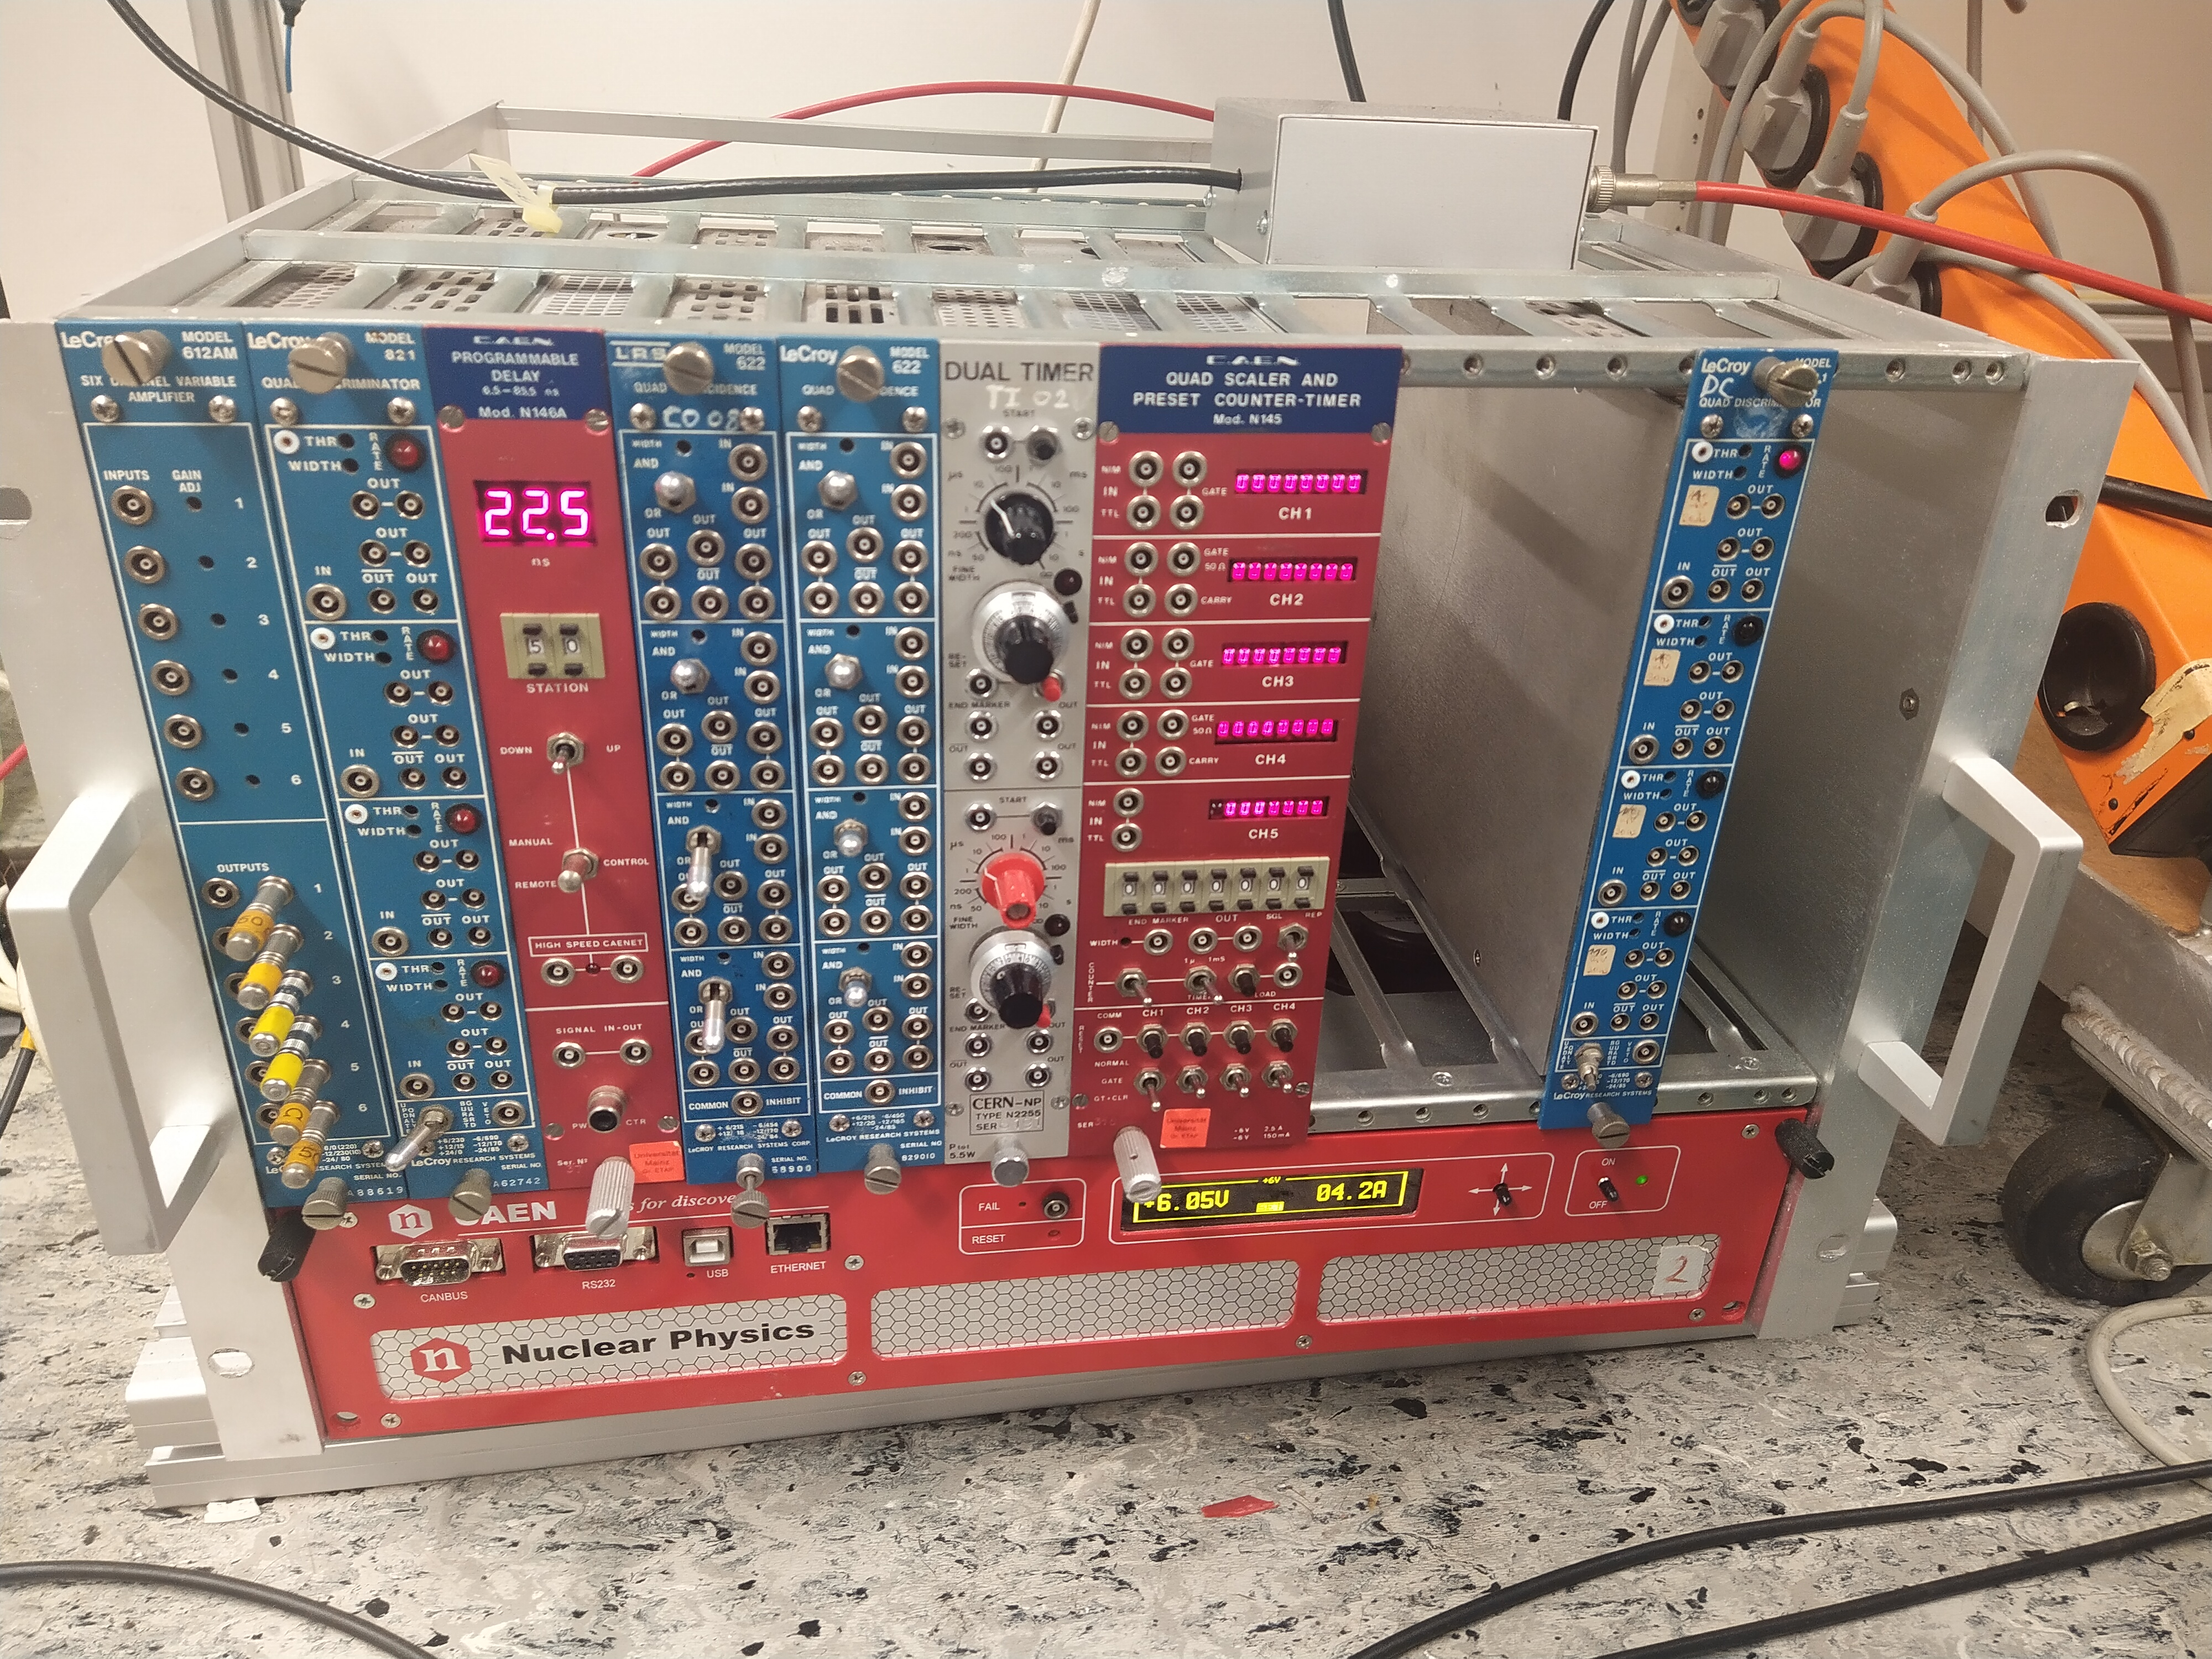
\includegraphics[width=\linewidth]{./fig/pic.png}
\caption{Picture of the electronic modules. (1) Amplifier input, the amplification can be tuned using a screwdriver in the holes left of the standerdized inputs. (2) Amplifier outputs. (3) Discriminators, parameters of the output gate can be tuned in the same way as the amplification for (1). (4) Programmable delay, the delay here is fixed at \SI{22.5}{\nano\second}. (5) Coincidence modules, they can be set to function in different ways (notably \textbf{AND} or \textbf{OR}). (6) Monoflop unit. (7) Digital counter, can be set to count over a period of time or to count ``normally'' (plug and count).}
\end{figure}
